% !TEX root = ../main.tex
\section{Experiment} \label{sec::experiment}
A particle accelerator is a machine that can accelerate charged particles to very high speeds.
It contains them in well-defined beams via an electromagnetic field, providing an environment in which controlled collisions can occur.
This is done so that we can study the small particles that result from these impacts~\cite{leduff2005longitudinal}.

Since a particle cannot reach the speed of light in a vacuum, it is more useful to measure its energy and momentum.
This is done in electronvolts (eV), which is the kinetic energy gained by a single electron accelerating from rest through an electric potential difference of one volt in vacuum~\cite{codata2015ev}.
For simplicity, it is usually measured in terms of MeV, GeV, TeV, etc.

As of the time of writing, two types of accelerators are mainly used to study particle physics:
Circular and linear accelerators (linacs).
The latter accelerate particles by attracting them onto charged plates, switching charge after the particles pass to repel them, pushing them to the next plate and repeating the process.
Linacs generally achieve lower momenta than their circular counterparts, but offer the advantage of a continuous stream of particles, thus achieving higher luminosity~\cite{pinchoff2005introduction}.

% !TEX root = ../main.tex
\subsection{CEBAF} \label{ssec::cebaf}
    \begin{figure}[b!]
        \centering\frame{
        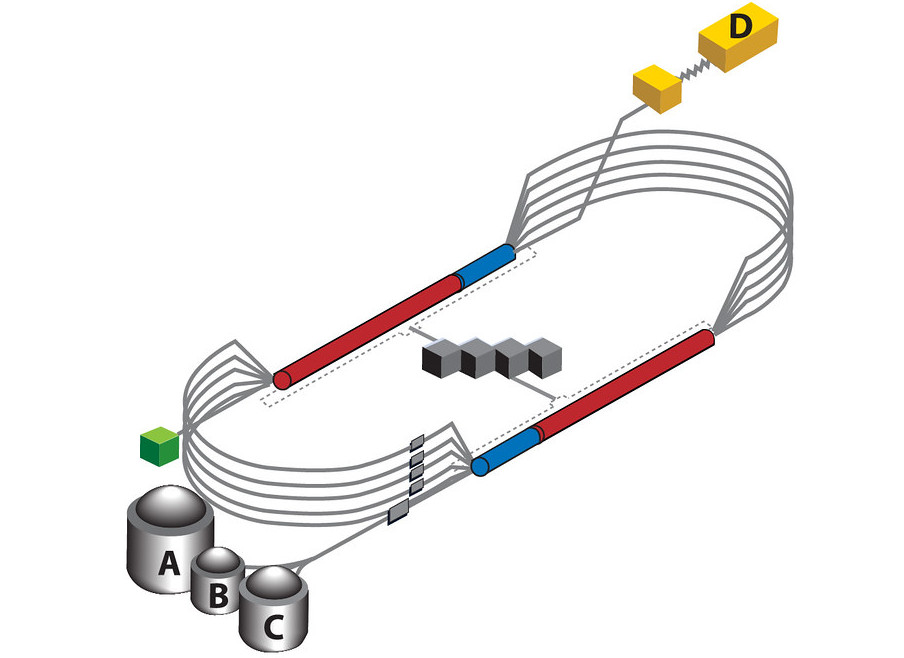
\includegraphics[width=\textwidth]{11experiment/img/10cebaf_diagram.jpg}}
        \caption[CEBAF.]{Simplified representation of CEBAF.
        Source: \hyperlink{https://www.jlab.org/}{jlab.org}.}
        \label{fig::cebaf}
    \end{figure}
    
    CEBAF is a pair of $1.4$-km antiparallel superconducting radio-frequency (RF) linear accelerators (linacs) built 8 meters below the surface.
    Both accelerators are joined by two $180\degree$ arcs, which have a radius of $80$ meters \cite{leemann2001} each.
    A figure detailing the design of CEBAF is available in Figure \ref{fig::cebaf}.

    The recirculating arcs are composed of five separate beamline sections, allowing the beam to cross both linacs up to five times.
    For each linac, the gain in energy of the beam varies between $0.8$ GeV up to $1.2$ GeV, giving it a final energy of about $12$ GeV.
    CEBAF is designed for the experimental study of the structure of mesons, nucleons, and nuclei through the high energy electron beam \cite{rode2010}.

% !TEX root = ../main.tex
\subsection{CLAS} \label{ssec::clas}
    \begin{figure}[htbp]
        \centering
        \fbox{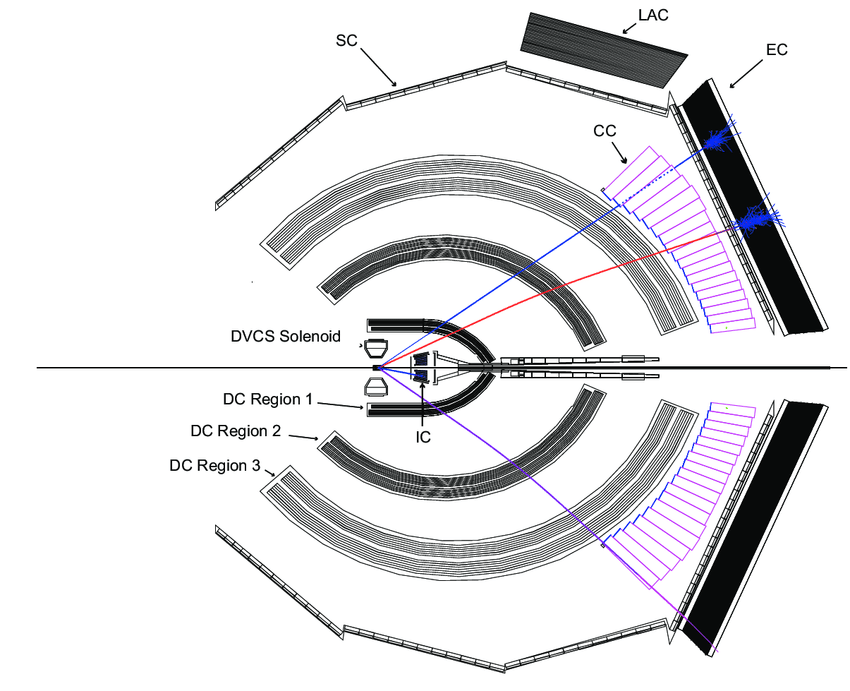
\includegraphics[width=0.8\textwidth]{11experiment/img/20clas.png}}
        \caption{\label{fig::clas} Schematic of CLAS. \\
        Source: \cite{bedlinskiy2014pi0}.}
    \end{figure}

    Particularly, in Hall B, the detector utilised up to 2005 (\textbf{TODO: PENDING CITATION}) is the CEBAF Large Accelerator Spetrometer (CLAS), where each particle-target collision --- denominated event --- is captured for analysis.
    This is done in an order of up to several thousand events per second, and the recorded data is later transferred to a farm of computing processors
    for High Energy Physics (HEP) analysis to be done on it.

    The design of CLAS is based on a toroidal magnetic field.
    This provides a momentum resolution of $\delta p/p \leq 0.5\%$~\cite{mestayer2000dc}.
    The design also has full azimuthal angle coverage and polar angle coverage from 8$\deg$ to 142$\deg$ relative to the direction of the incoming beam~\cite{mecking2003cebaf}.
    Thanks to this large angle acceptance for charged particles, CLAS is well suited for experiments that require the detection of two or more particles.
    
    CLAS is divided into six identical sectors, where each is an independent spectrometer.
    5-meter long superconducting coils of toroidal magnets separate each sector.
    These magnets produce a toroidal magnetic field which bends particles in only the polar direction.
    
    In CLAS experiments, it is standard for the field to force the particles to be in-bending compared to the direction of the beam.
    This is the case for the experiment that forms the basis of this work, EG2.
    
    A diagram of CLAS can be seen in figure \ref{fig::clas}.
    The inbending trajectories of the charged particles (in red and purple) can be seen.

    The particle detection system consists of five detectors which are designed to measure different properties of the particles from the reaction.
    These are Drift Chambers (DC), Cherekov Counters (CC), Time-Of-Flight (TOF), Scintillation Counters (SC), and Electromagnetic Calorimeters (EC).
    Each of these will be detailed in the following subsections.
    
    \input{11experiment/21dc}
    \input{11experiment/22cc}
    \input{11experiment/23sc}
    \input{11experiment/24ec}

\input{11experiment/30eg2}
